\documentclass{standalone}
\usepackage{tikz}
\usetikzlibrary{patterns, positioning}


\begin{document}
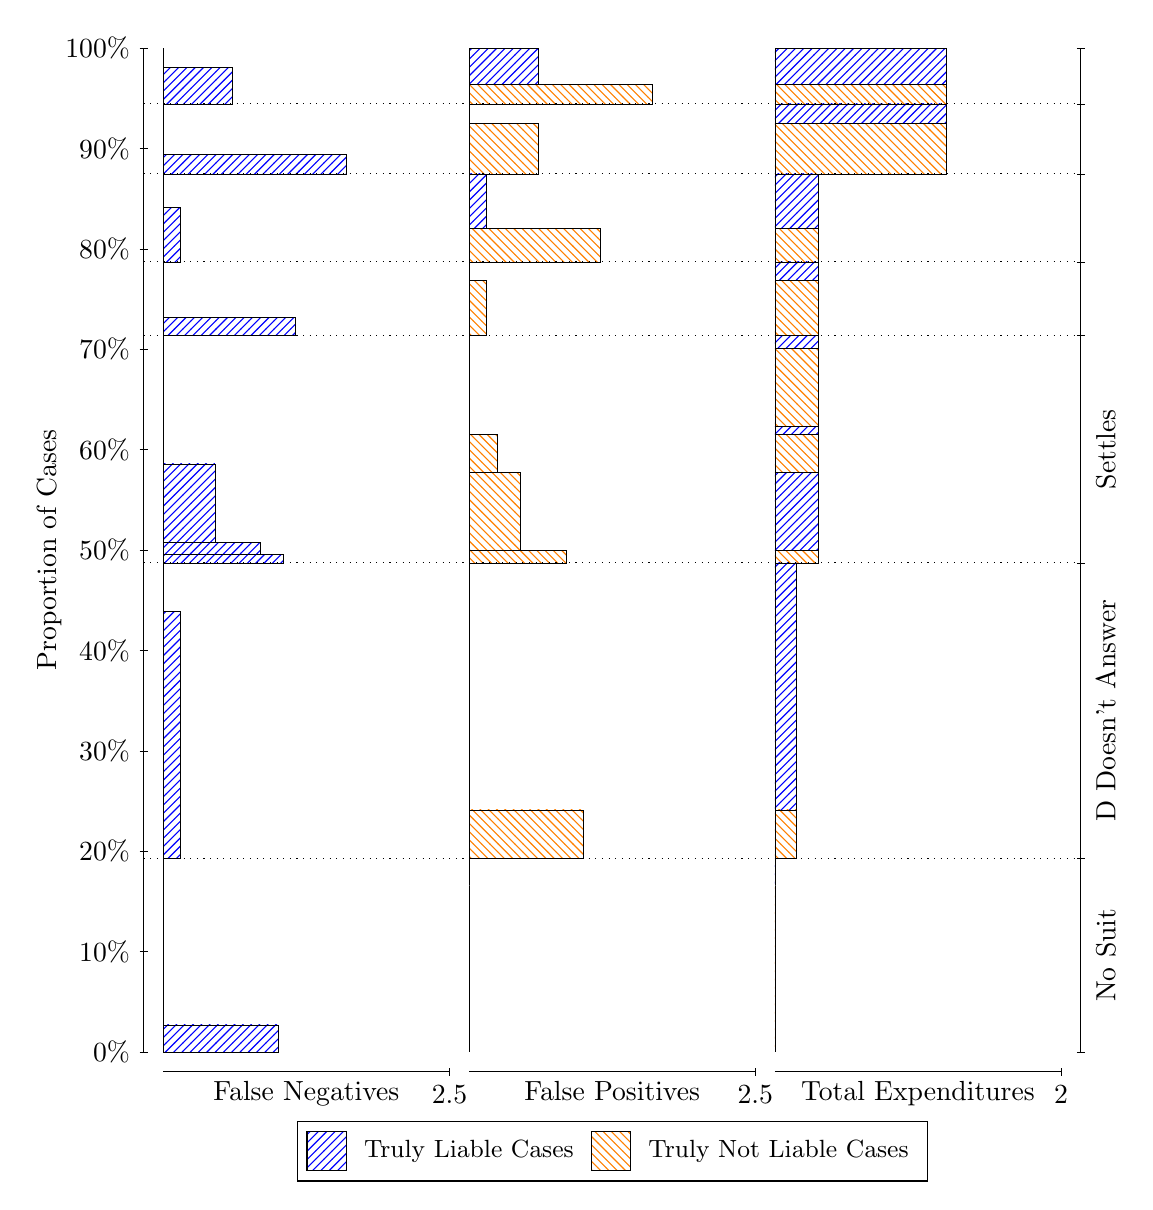
\begin{tikzpicture}
\draw[black, very thin] (1.5,1.75) -- (1.5,14.5);
\node[rotate=90, text=black, anchor=center] at (0.3, 8.125) {Proportion of Cases};
\draw[black, very thin] (1.45,1.75) -- (1.55,1.75);
\node[text=black, anchor=east] at (1.45, 1.75) {0\%};
\draw[black, very thin] (1.45,3.025) -- (1.55,3.025);
\node[text=black, anchor=east] at (1.45, 3.025) {10\%};
\draw[black, very thin] (1.45,4.3) -- (1.55,4.3);
\node[text=black, anchor=east] at (1.45, 4.3) {20\%};
\draw[black, very thin] (1.45,5.575) -- (1.55,5.575);
\node[text=black, anchor=east] at (1.45, 5.575) {30\%};
\draw[black, very thin] (1.45,6.85) -- (1.55,6.85);
\node[text=black, anchor=east] at (1.45, 6.85) {40\%};
\draw[black, very thin] (1.45,8.125) -- (1.55,8.125);
\node[text=black, anchor=east] at (1.45, 8.125) {50\%};
\draw[black, very thin] (1.45,9.4) -- (1.55,9.4);
\node[text=black, anchor=east] at (1.45, 9.4) {60\%};
\draw[black, very thin] (1.45,10.675) -- (1.55,10.675);
\node[text=black, anchor=east] at (1.45, 10.675) {70\%};
\draw[black, very thin] (1.45,11.95) -- (1.55,11.95);
\node[text=black, anchor=east] at (1.45, 11.95) {80\%};
\draw[black, very thin] (1.45,13.225) -- (1.55,13.225);
\node[text=black, anchor=east] at (1.45, 13.225) {90\%};
\draw[black, very thin] (1.45,14.5) -- (1.55,14.5);
\node[text=black, anchor=east] at (1.45, 14.5) {100\%};

\draw[black, very thin] (13.4,1.75) -- (13.4,14.5);
\draw[black, very thin] (13.35,1.75) -- (13.45,1.75);
\node[anchor=west] at (13.35, 1.75) {};
\draw[black, very thin] (13.35,4.2063) -- (13.45,4.2063);
\node[anchor=west] at (13.35, 4.2063) {};
\draw[black, very thin] (13.35,7.9612) -- (13.45,7.9612);
\node[anchor=west] at (13.35, 7.9612) {};
\draw[black, very thin] (13.35,10.848) -- (13.45,10.848);
\node[anchor=west] at (13.35, 10.848) {};
\draw[black, very thin] (13.35,11.784) -- (13.45,11.784);
\node[anchor=west] at (13.35, 11.784) {};
\draw[black, very thin] (13.35,12.901) -- (13.45,12.901);
\node[anchor=west] at (13.35, 12.901) {};
\draw[black, very thin] (13.35,13.791) -- (13.45,13.791);
\node[anchor=west] at (13.35, 13.791) {};
\draw[black, very thin] (13.35,14.5) -- (13.45,14.5);
\node[anchor=west] at (13.35, 14.5) {};

\draw[black, very thin, pattern color=blue, pattern=north east lines] (1.75,1.75) rectangle (3.2033,2.0934);
\draw[black, very thin, pattern color=orange, pattern=north west lines] (1.75,2.0934) rectangle (1.75,4.2063);
\draw[black, very thin, pattern color=blue, pattern=north east lines] (1.75,4.2063) rectangle (1.968,7.3418);
\draw[black, very thin, pattern color=orange, pattern=north west lines] (1.75,7.3418) rectangle (1.75,7.9612);
\draw[black, very thin, pattern color=blue, pattern=north east lines] (1.75,7.9612) rectangle (3.276,8.0672);
\draw[black, very thin, pattern color=blue, pattern=north east lines] (1.75,8.0672) rectangle (2.9853,8.226);
\draw[black, very thin, pattern color=blue, pattern=north east lines] (1.75,8.226) rectangle (2.404,9.2177);
\draw[black, very thin, pattern color=orange, pattern=north west lines] (1.75,9.2177) rectangle (1.75,10.848);
\draw[black, very thin, pattern color=blue, pattern=north east lines] (1.75,10.848) rectangle (3.4213,11.084);
\draw[black, very thin, pattern color=orange, pattern=north west lines] (1.75,11.084) rectangle (1.75,11.784);
\draw[black, very thin, pattern color=blue, pattern=north east lines] (1.75,11.784) rectangle (1.968,12.479);
\draw[black, very thin, pattern color=orange, pattern=north west lines] (1.75,12.479) rectangle (1.75,12.901);
\draw[black, very thin, pattern color=blue, pattern=north east lines] (1.75,12.901) rectangle (4.0753,13.15);
\draw[black, very thin, pattern color=orange, pattern=north west lines] (1.75,13.15) rectangle (1.75,13.791);
\draw[black, very thin, pattern color=blue, pattern=north east lines] (1.75,13.791) rectangle (2.622,14.251);
\draw[black, very thin, pattern color=orange, pattern=north west lines] (1.75,14.251) rectangle (1.75,14.5);
\draw[black, very thin, pattern color=orange, pattern=north west lines] (5.6333,1.75) rectangle (5.6333,3.8629);
\draw[black, very thin, pattern color=blue, pattern=north east lines] (5.6333,3.8629) rectangle (5.6333,4.2063);
\draw[black, very thin, pattern color=orange, pattern=north west lines] (5.6333,4.2063) rectangle (7.0867,4.8257);
\draw[black, very thin, pattern color=blue, pattern=north east lines] (5.6333,4.8257) rectangle (5.6333,7.9612);
\draw[black, very thin, pattern color=orange, pattern=north west lines] (5.6333,7.9612) rectangle (6.8687,8.12);
\draw[black, very thin, pattern color=orange, pattern=north west lines] (5.6333,8.12) rectangle (6.2873,9.1117);
\draw[black, very thin, pattern color=orange, pattern=north west lines] (5.6333,9.1117) rectangle (5.9967,9.5917);
\draw[black, very thin, pattern color=blue, pattern=north east lines] (5.6333,9.5917) rectangle (5.6333,10.848);
\draw[black, very thin, pattern color=orange, pattern=north west lines] (5.6333,10.848) rectangle (5.8513,11.548);
\draw[black, very thin, pattern color=blue, pattern=north east lines] (5.6333,11.548) rectangle (5.6333,11.784);
\draw[black, very thin, pattern color=orange, pattern=north west lines] (5.6333,11.784) rectangle (7.3047,12.206);
\draw[black, very thin, pattern color=blue, pattern=north east lines] (5.6333,12.206) rectangle (5.8513,12.901);
\draw[black, very thin, pattern color=orange, pattern=north west lines] (5.6333,12.901) rectangle (6.5053,13.542);
\draw[black, very thin, pattern color=blue, pattern=north east lines] (5.6333,13.542) rectangle (5.6333,13.791);
\draw[black, very thin, pattern color=orange, pattern=north west lines] (5.6333,13.791) rectangle (7.9587,14.04);
\draw[black, very thin, pattern color=blue, pattern=north east lines] (5.6333,14.04) rectangle (6.5053,14.5);
\draw[black, very thin, pattern color=orange, pattern=north west lines] (9.5167,1.75) rectangle (9.5167,3.8629);
\draw[black, very thin, pattern color=blue, pattern=north east lines] (9.5167,3.8629) rectangle (9.5167,4.2063);
\draw[black, very thin, pattern color=orange, pattern=north west lines] (9.5167,4.2063) rectangle (9.7892,4.8257);
\draw[black, very thin, pattern color=blue, pattern=north east lines] (9.5167,4.8257) rectangle (9.7892,7.9612);
\draw[black, very thin, pattern color=orange, pattern=north west lines] (9.5167,7.9612) rectangle (10.062,8.12);
\draw[black, very thin, pattern color=blue, pattern=north east lines] (9.5167,8.12) rectangle (10.062,9.1116);
\draw[black, very thin, pattern color=orange, pattern=north west lines] (9.5167,9.1116) rectangle (10.062,9.5917);
\draw[black, very thin, pattern color=blue, pattern=north east lines] (9.5167,9.5917) rectangle (10.062,9.6977);
\draw[black, very thin, pattern color=orange, pattern=north west lines] (9.5167,9.6977) rectangle (10.062,10.689);
\draw[black, very thin, pattern color=blue, pattern=north east lines] (9.5167,10.689) rectangle (10.062,10.848);
\draw[black, very thin, pattern color=orange, pattern=north west lines] (9.5167,10.848) rectangle (10.062,11.548);
\draw[black, very thin, pattern color=blue, pattern=north east lines] (9.5167,11.548) rectangle (10.062,11.784);
\draw[black, very thin, pattern color=orange, pattern=north west lines] (9.5167,11.784) rectangle (10.062,12.206);
\draw[black, very thin, pattern color=blue, pattern=north east lines] (9.5167,12.206) rectangle (10.062,12.901);
\draw[black, very thin, pattern color=orange, pattern=north west lines] (9.5167,12.901) rectangle (11.697,13.542);
\draw[black, very thin, pattern color=blue, pattern=north east lines] (9.5167,13.542) rectangle (11.697,13.791);
\draw[black, very thin, pattern color=orange, pattern=north west lines] (9.5167,13.791) rectangle (11.697,14.04);
\draw[black, very thin, pattern color=blue, pattern=north east lines] (9.5167,14.04) rectangle (11.697,14.5);
\draw[black, dotted] (1.5,4.2063) -- (13.4,4.2063);
\draw[black, dotted] (1.5,7.9612) -- (13.4,7.9612);
\draw[black, dotted] (1.5,10.848) -- (13.4,10.848);
\draw[black, dotted] (1.5,11.784) -- (13.4,11.784);
\draw[black, dotted] (1.5,12.901) -- (13.4,12.901);
\draw[black, dotted] (1.5,13.791) -- (13.4,13.791);
\draw[black, very thin] (1.75,1.5) -- (5.3833,1.5);
\node[text=black, anchor=north] at (3.5667, 1.5) {False Negatives};
\draw[black, very thin] (5.3833,1.45) -- (5.3833,1.55);
\node[text=black, anchor=north] at (5.3833, 1.45) {2.5};

\draw[black, very thin] (5.6333,1.5) -- (9.2667,1.5);
\node[text=black, anchor=north] at (7.45, 1.5) {False Positives};
\draw[black, very thin] (9.2667,1.45) -- (9.2667,1.55);
\node[text=black, anchor=north] at (9.2667, 1.45) {2.5};

\draw[black, very thin] (9.5167,1.5) -- (13.15,1.5);
\node[text=black, anchor=north] at (11.333, 1.5) {Total Expenditures};
\draw[black, very thin] (13.15,1.45) -- (13.15,1.55);
\node[text=black, anchor=north] at (13.15, 1.45) {2};

\node[text=black, centered, rotate=90] at (13.72, 2.9781) {No Suit};
\node[text=black, centered, rotate=90] at (13.72, 6.0837) {D Doesn't Answer};
\node[text=black, centered, rotate=90] at (13.72, 9.4047) {Settles};





\draw (7.449999999999999,1.5) node[draw=none] (baseCoordinate) {};
\begin{scope}[align=center]
        \matrix[scale=0.5, draw=black, below=0.5cm of baseCoordinate, nodes={draw}, column sep=0.1cm]{
            \node[rectangle, draw, minimum width=0.5cm, minimum height=0.5cm, pattern color=blue, pattern=north east lines] {}; &
            \node[draw=none, font=\small, text=black] (B) {Truly Liable Cases}; &
            \node[rectangle, draw, minimum width=0.5cm, minimum height=0.5cm, pattern color=orange, pattern=north west lines] {}; &
            \node[draw=none, font=\small, text=black] (B) {Truly Not Liable Cases}; \\
            };
\end{scope}

\end{tikzpicture}
\end{document}